\textcolor{red}{Parlare dei big data, in particolare dei problemi con la quantità di dati e necessità di mettere ordine, dare significato\\
	prendere spunto da articolo and what can context do for data\\
	trovare grafici\\
	obiettivi della tesi}

Negli ultimi anni si è assistito a un'enorme diffusione di Internet e soprattutto a una varietà di dispositivi con i quali è possibile accederci. Agli albori esistevano solamente PC desktop con i quali poter visitare pagine per lo più statiche.

Ai giorni d'oggi invece sono disponibili dispositivi come smartphone e tablet che ci permettono di essere sempre connessi. Grazie al fatto che sono estremamente portatili e semplici sono ormai diventati oggetti indispensabili nella vita quotidiana. L'anno scorso è stato generato più traffico proveniente dagli smartphone rispetto ai PC (Figura \ref{fig:traffico-tipologia-dispositivo}). L'incremento della velocità delle connessioni e il progresso tecnologico ha fatto sì che sia possibile consultare qualsiasi tipo di informazione su internet, dal semplice testo fino a immagini, video, ecc.

\begin{figure}[ht]
	\centering
	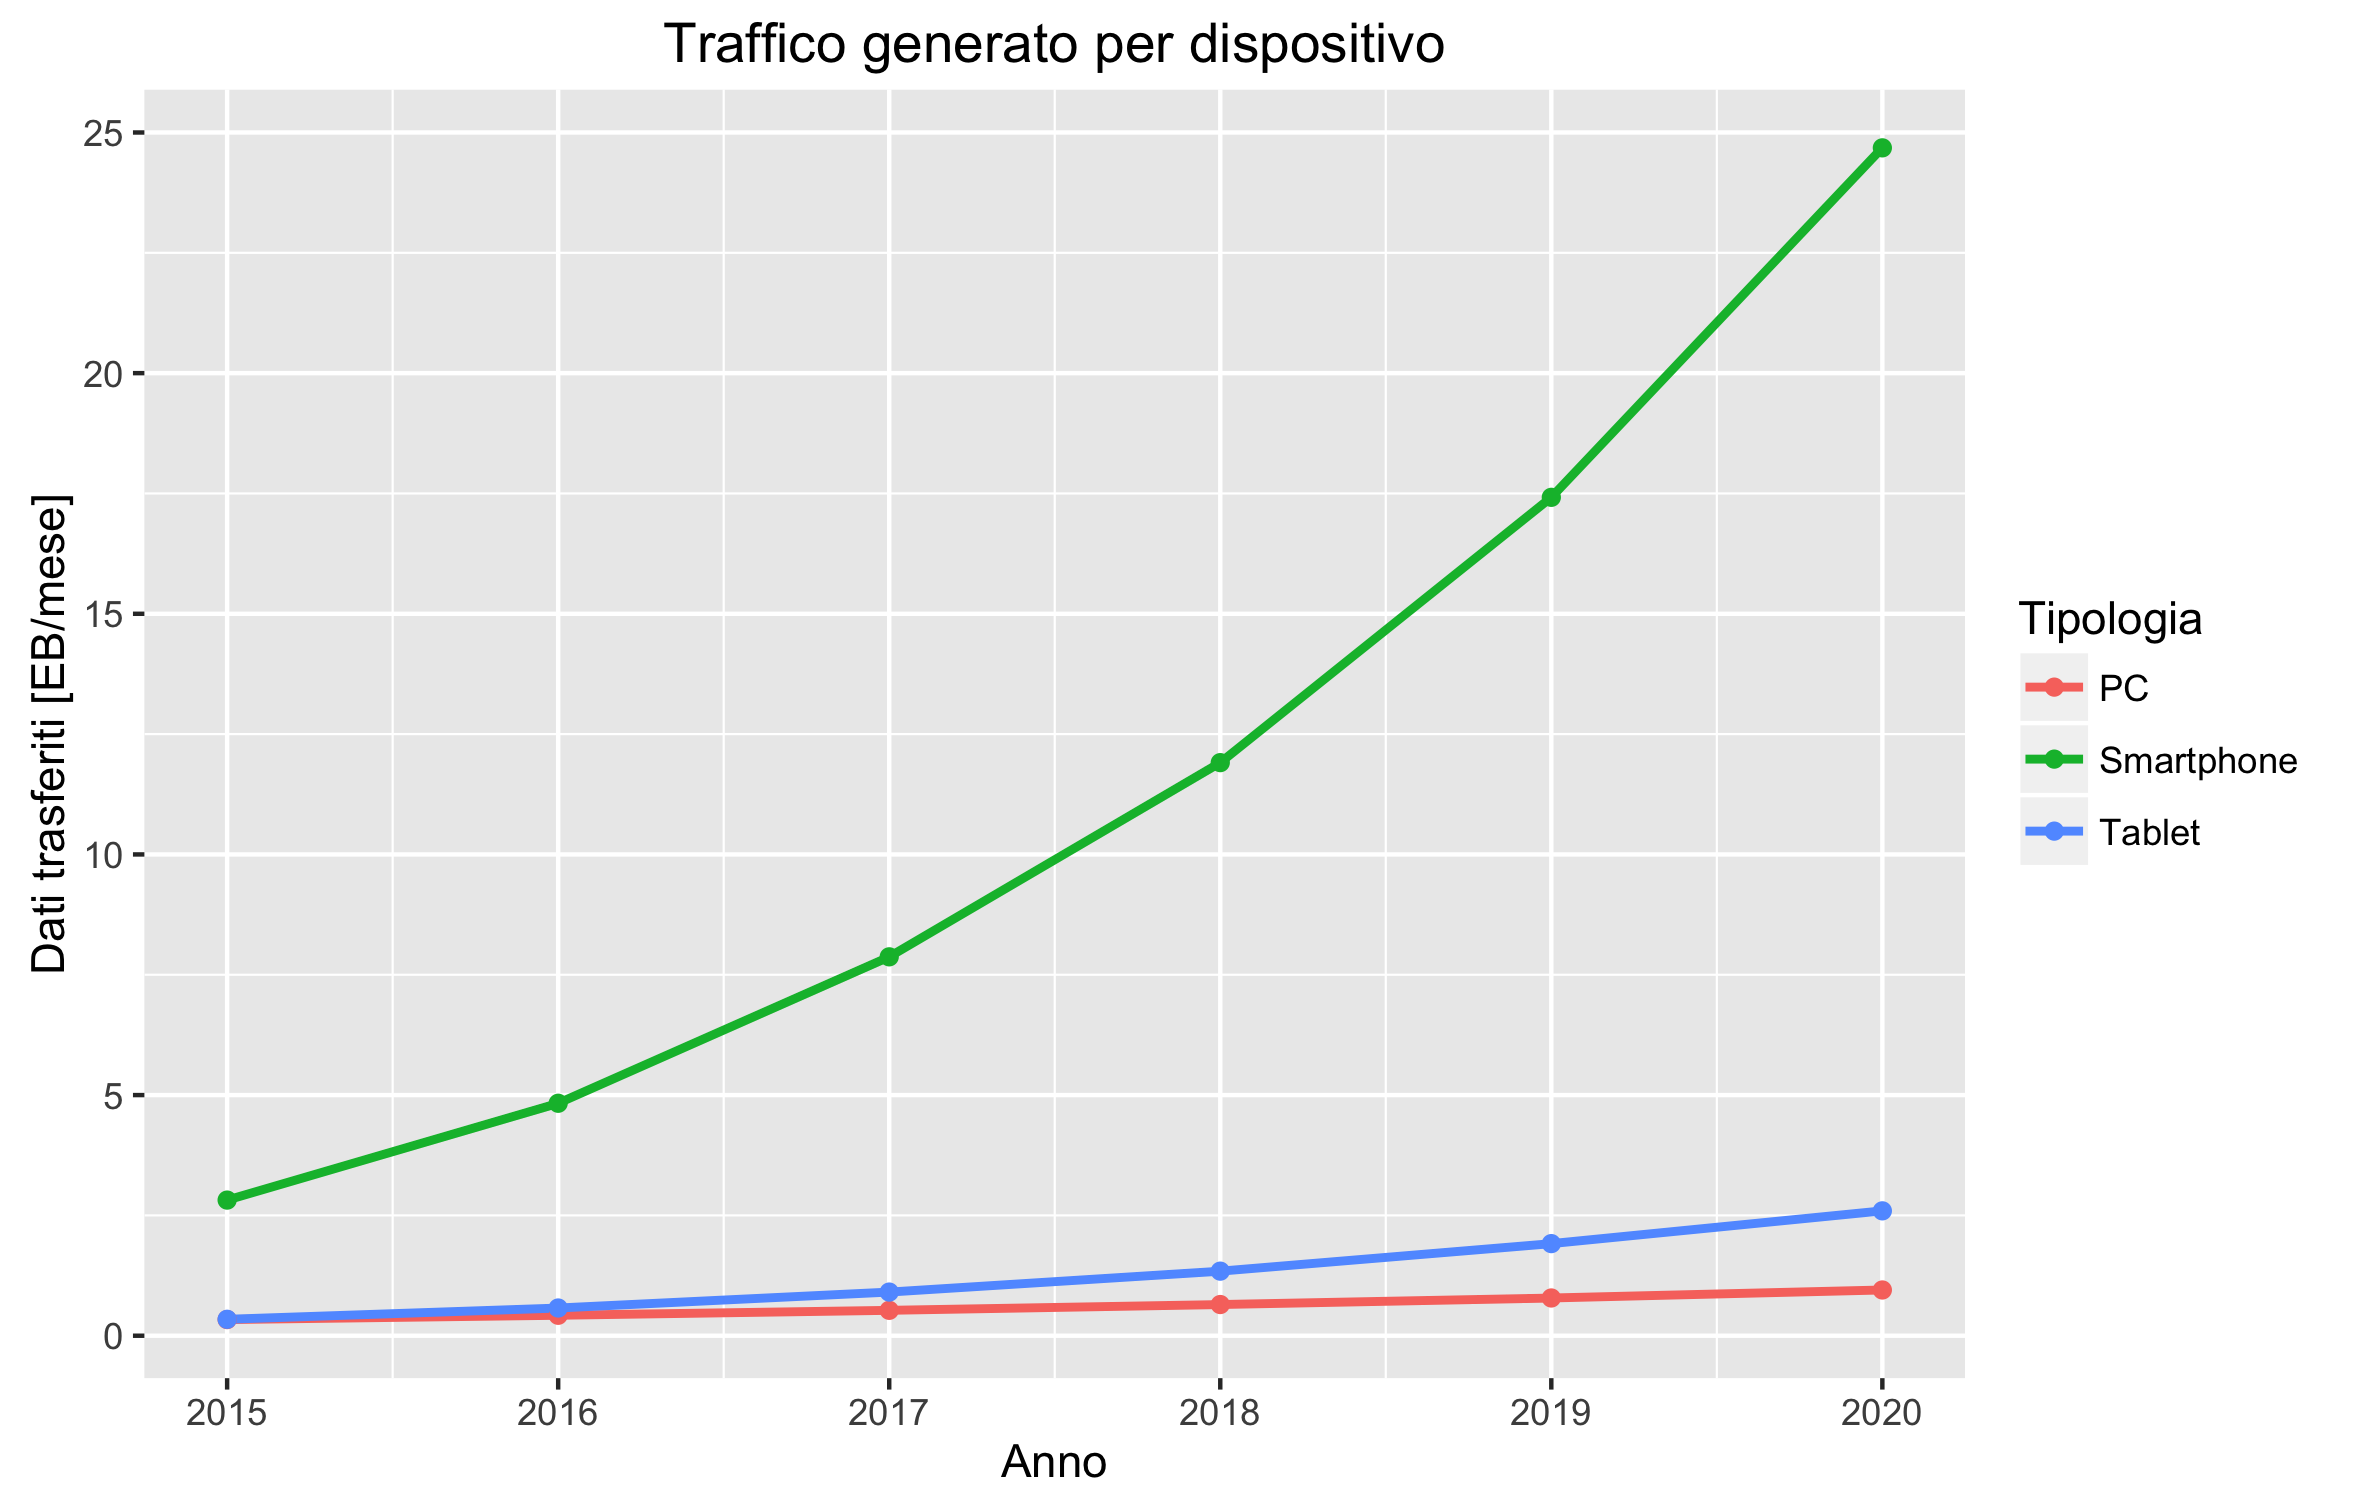
\includegraphics[width=\textwidth]{1-introduzione/Immagini/traffico-dispositivi.png}
	\caption[Traffico generato per tipologia di dispositivo]{Traffico generato per tipologia di dispositivo (fonte: Cisco, 2016)\label{fig:traffico-tipologia-dispositivo}}
\end{figure}

Si è persa anche la tradizione che sia un gestore a pubblicare contenuti in quanto ormai sono direttamente gli utenti a produrre la maggior parte delle informazioni disponibili (Figura \ref{fig:analisi-dati-generati}). Questo fenomeno è stato accentuato con la creazione dei \emph{social network}, che permettono di creare collegamenti tra le persone dove è possibile condividere qualunque cosa che ognuno trova interessante. Gli utenti vengono così coinvolti nella creazione di contenuti che, grazie anche alla dotazione di fotocamera ad alta risoluzione nei propri dispositivi, possono essere multimediali. 

\begin{figure}[ht]
	\centering
	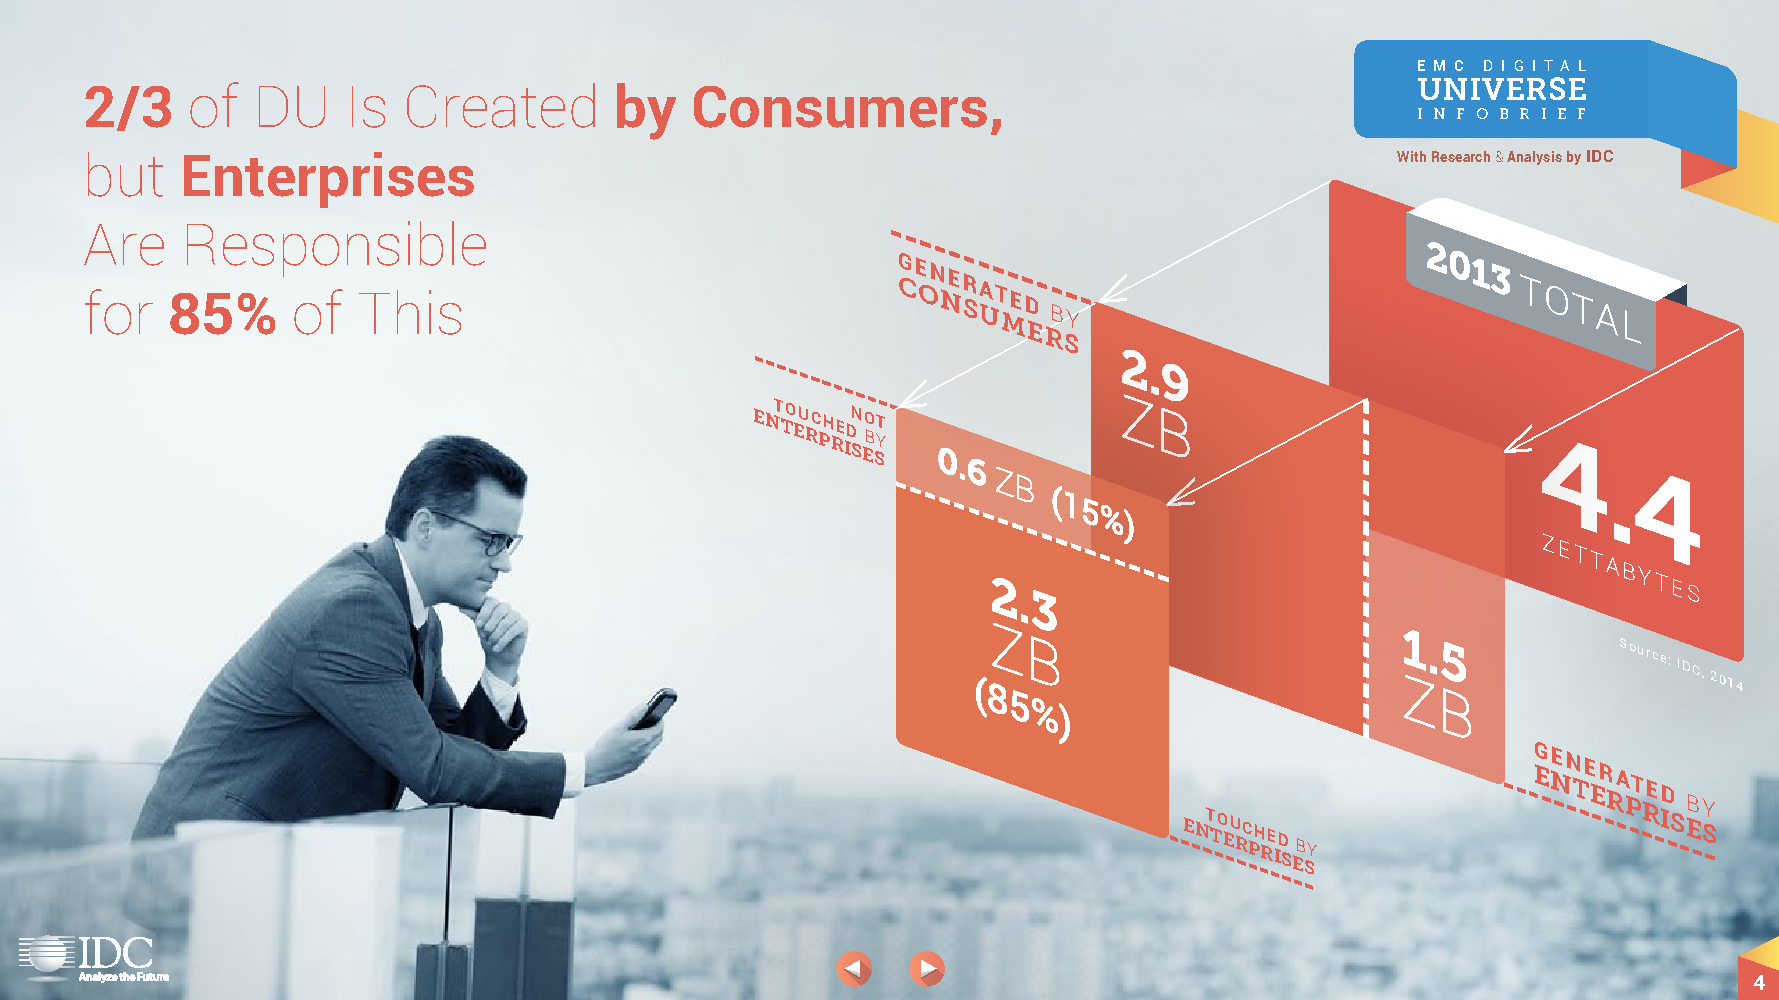
\includegraphics[width=\textwidth]{1-introduzione/Immagini/dati-generati-consumer.pdf}
	\caption[Analisi della quantità di dati generati]{Analisi della quantità di dati generati (fonte: IDC, 2014)\label{fig:analisi-dati-generati}}
\end{figure}

Come si può notare in Figura \ref{fig:traffico-categoria-applicazione} il traffico video e audio è in costante aumento. In particolare il traffico di video sovrasta tutti gli altri, anche a causa della maggior dimensioni di questi contenuti. Questo fenomeno è dovuto alla crescita dei servizi che permettono lo \emph{streaming} dei contenuti multimediali come YouTube\footnote{YouTube: \url{https://www.youtube.com}} o Netflix\footnote{Netflix: \url{https://www.netflix.com}}.

\begin{figure}[ht]
	\centering
	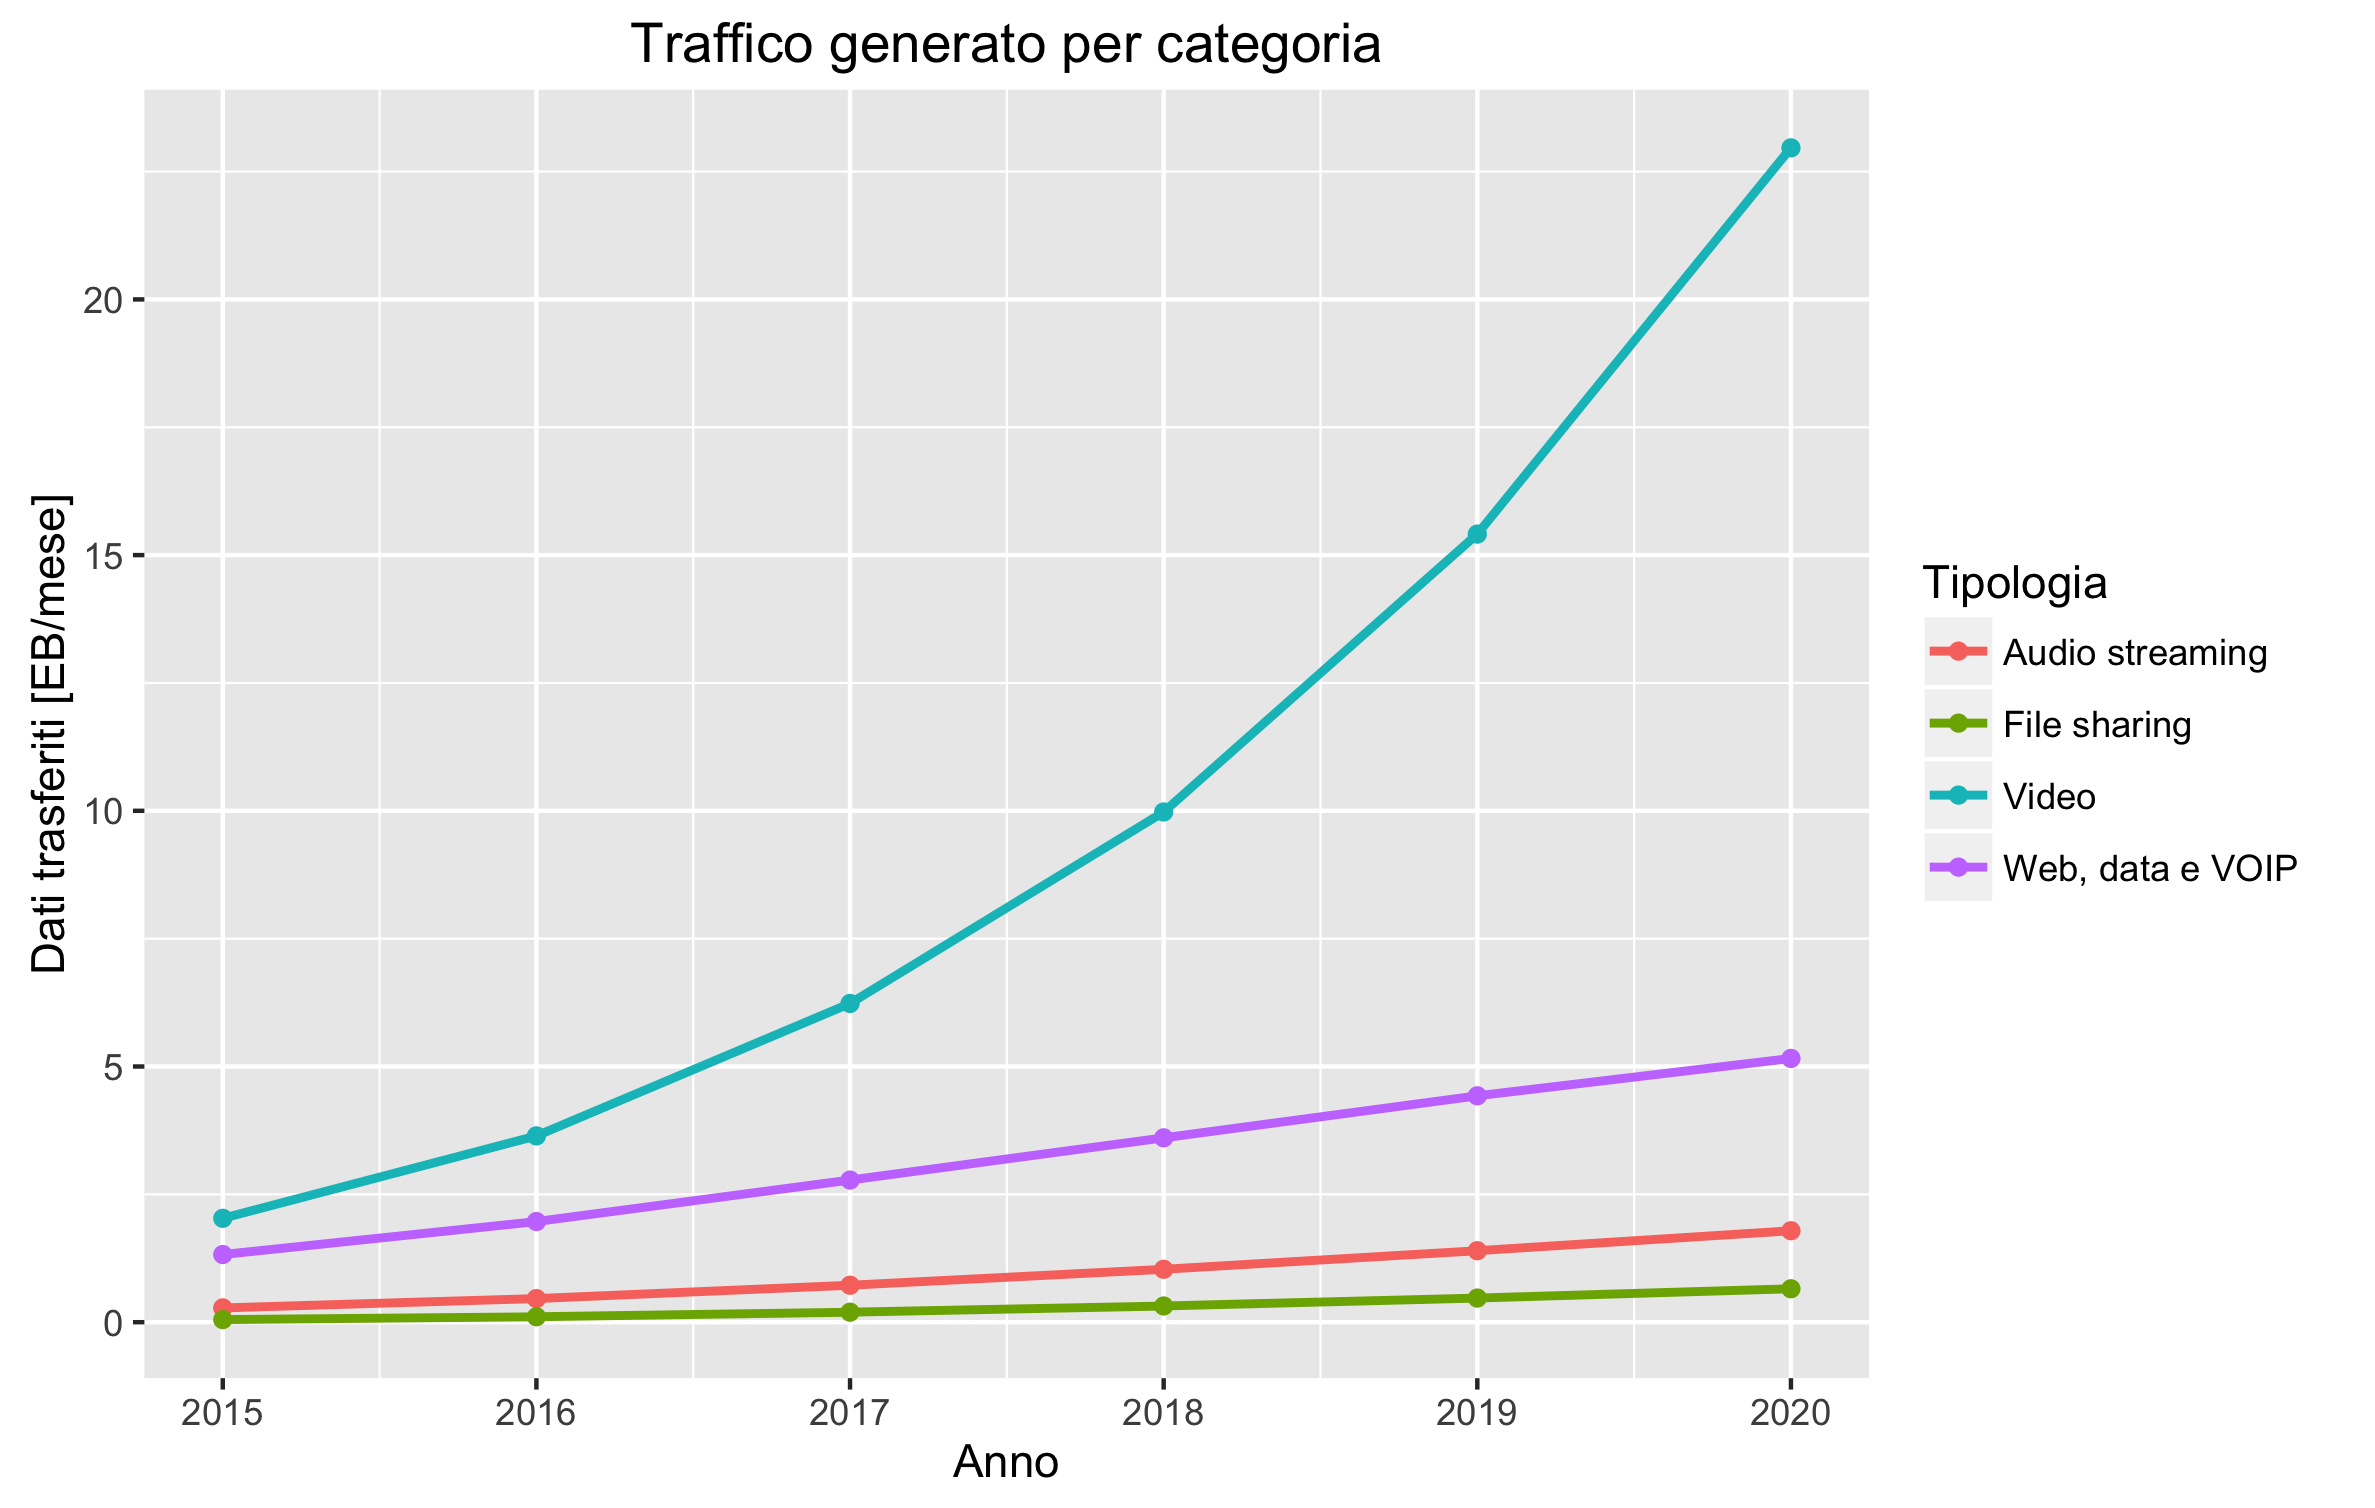
\includegraphics[width=\textwidth]{1-introduzione/Immagini/traffico-categoria.png}
	\caption[Traffico generato per categoria di applicazione]{Traffico generato per categoria di applicazione (fonte: Cisco, 2016)\label{fig:traffico-categoria-applicazione}}
\end{figure}

Internet è diventato una fonte immensa di informazioni che è destinato sempre ad aumentare (Figura \ref{fig:statistiche-iot}). Un recente trend è relativo ai dispositivi connessi, definito \emph{Internet of Things}. L'idea è che qualsiasi dispositivo può essere connesso a Internet per generare informazioni, in particolare tutti quelli provvisti di \emph{sensori} che possono fornire dati sullo stato dell'ambiente nel quale si trovano.

\begin{figure}[ht]
	\centering
	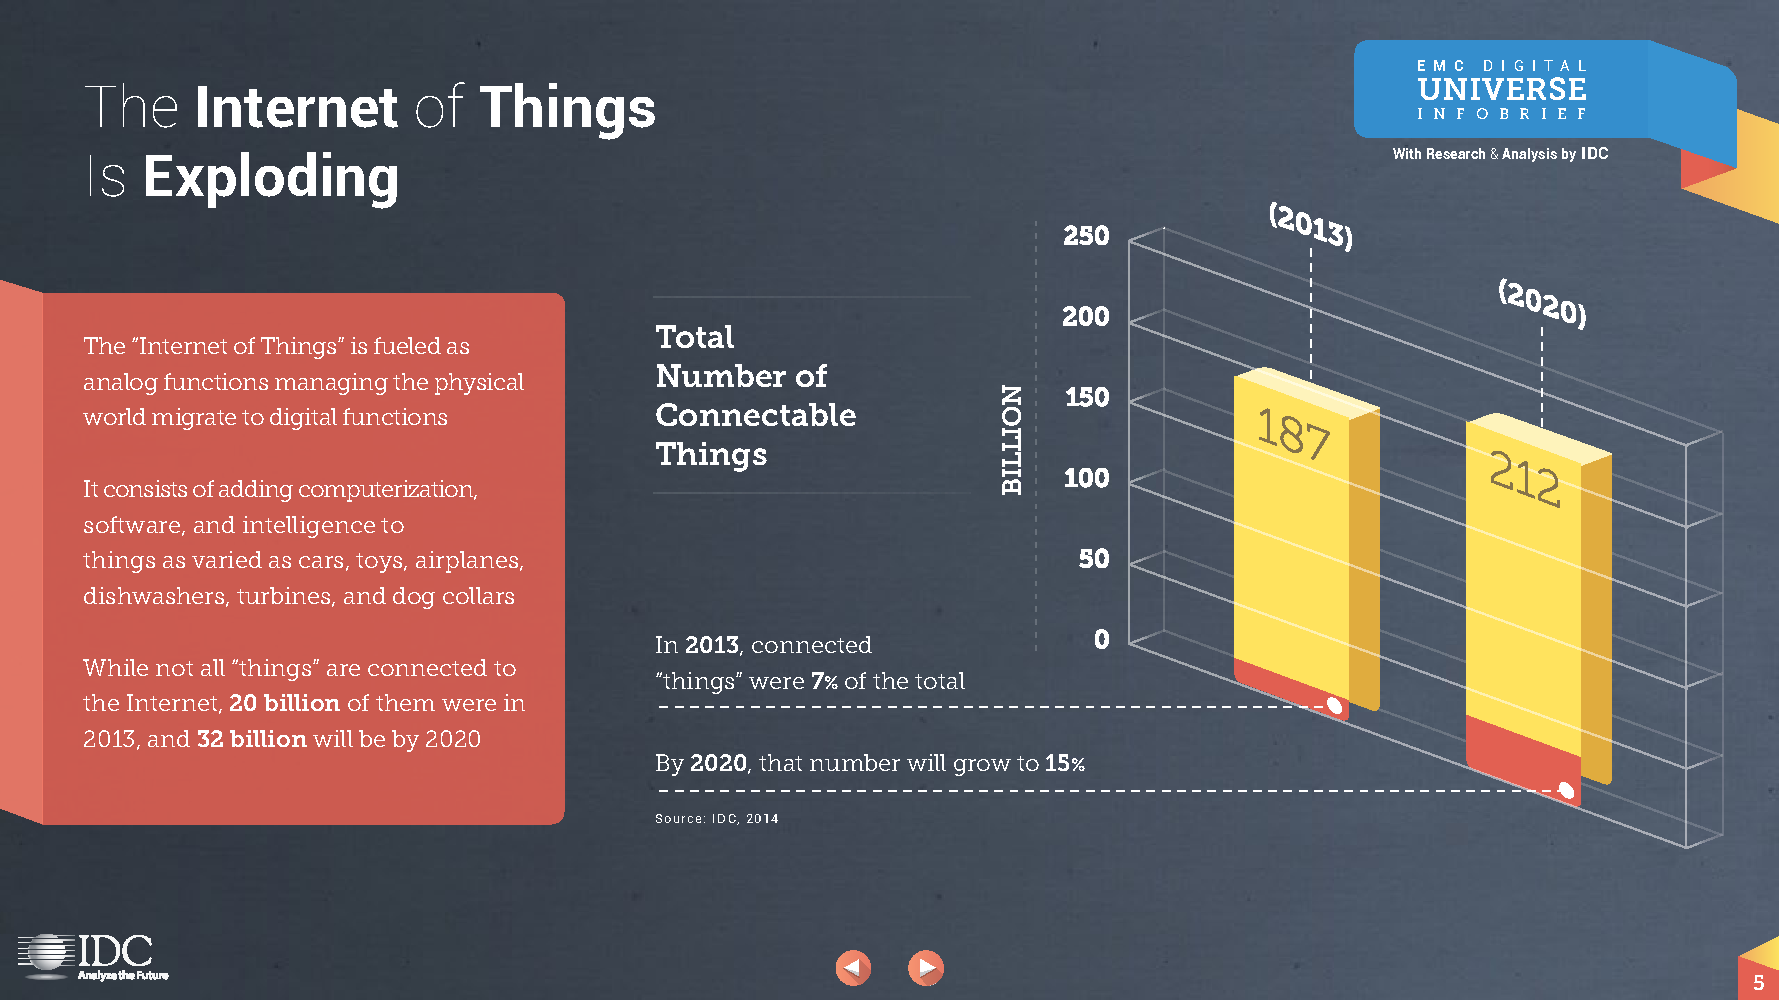
\includegraphics[width=\textwidth]{1-introduzione/Immagini/iot-trend.pdf}
	\caption[Statistiche sull'Internet of Things]{Statistiche sull'Internet of Things (fonte: IDC, 2014)\label{fig:statistiche-iot}}
\end{figure}

%Inizio parte del contesto
Questa è la \emph{Information Age}, cioè il fenomeno dove la conoscenza è alla base della società e la tecnologia influenza il modo in cui operano le industrie e gli operatori dei servizi, permettendogli di agire in modo più efficiente e conveniente. Tutte queste informazioni permettono a chiunque di esplorarle secondo le proprie esigenze. 

Uno dei principali problemi che chiunque lavori coi dati vuole cercare di risolvere è ridurre lo \virgolette{information noise} migliorando la precisione delle informazioni da mostrare che meglio si adattano ai requisiti.

\upe frequente che le informazioni non vengano acquisite unicamente da una base di dati bensì provengono da più fonti, anche di tipologie diverse tra loro (es.: relazionali, XML, ec..). Basti pensare alla moltitudine di servizi presenti nel web.

Questo aumento della quantità di informazioni, se non propriamente controllato, può provocare un ammasso di dati che genera soltanto confusione piuttosto che fornire elementi utili, riducendo i benefici che invece si potrebbero ricavare da tutte queste informazioni. Tuttavia, distinguere le informazioni rilevanti da quelle che non lo sono è un compito tutt'altro che semplice: alcune informazioni potrebbero essere trattate in maniera differente, anche per lo stesso utente, che in diverse situazioni o posti ha bisogno di informazioni differenti. 

%Resta aperto il problema di come visualizzare le operazioni e come ricercare le info in modo semplice (Fornire interfaccia per permettere agli utenti di cercare le informazioni)

Una volta acquisite le informazioni nasce l'esigenza di definire regole su come mostrarle all'utente finale. Con la diffusione di dispositivi mobili sempre più sofisticati si è resa maggiormente necessaria un'esperienza utente semplice che lo guidi durante le sue attività .

%\textcolor{red}{Ruolo dell'user experience\\
%	parlare di come sia conveniente un meccanismo decori le informazioni testuali con contenuti aggiuntivi, come mappe, foto e altre cose dinamiche}

Per questo motivo ha assunto un ruolo di grande importanza l'esperienza d'uso dell'utente (User Experience). Infatti se un'applicazione non è ben formata e non è fruibile in modo semplice dall'utente, diminuisce la quantità di utenti dell'applicazione. Secondo Gary Illyes di Google circa il 61 percento\footnote{Search Engine Land Interview to Gary Illyes of Google: \url{http://searchengineland.com/google-may-add-mobile-user-experience-ranking-algorithm-205382}} degli utenti che incontrano problemi con siti e app su smartphone ne abbandonano l'utilizzo volontariamente. Per evitare questo problema è necessario prestare attenzione a come viene progettato tutto il flusso di navigazione dell'utente e a fornirgli i dati necessari per poter sfruttare al meglio l'applicazione e migliorare la conoscenza. L'aggiunta di elementi comprensibili in modo intuitivo come mappe e foto porta l'utente ad utilizzare altre aree della mente, come quella della memoria fotografica. In questo modo l'utente può facilmente acquisire conoscenza utilizzando diversi dati e diverse tipologie di visualizzazione.

%inizio parte di progetto
%{red}{Parlare degli obiettivi del progetto CAMUS}

Vengono dunque in soccorso i \emph{Mashup}, che permettono la realizzazione di interfacce grafiche estremamente dinamiche. In questo modo può essere facilmente rappresentato il contesto e definire un aspetto idoneo per le varie categorie di risultati. \textcolor{red}{Ogni categoria di informazioni ha le sue peculiarità e avere schemi diversi per categoria di dati ha il suo perché}
Per ogni categoria sono presenti alcuni dati comuni e altri che sono focalizzati sulla tipologia di dato che la definisce. Per questa varietà di dati è necessario avere la massima dinamicità nelle opzioni di visualizzazione per mostrare i risultati nel modo migliore. Utilizzando i mashup risulta più semplice definire queste visualizzazioni e sfruttare diverse fonti di dati per fornire informazioni all'utente finale.

\section{Struttura della tesi\label{sec:struttura-tesi}}

